\section{Metoder}
    \subsection{Synteser} 
    Med udgangspunkt i den fundne syntesevejledning \parencite{Ole2019} udføres syntesen for ethyl-- og propylparaben grundet deres respektive alkoholers lavewre farlighed end methanol. Af samme grund benyttes ethanol som opløsningsmiddel under oprensningen, idet der herved helt undgås eksponering for methanol hvilket drastisk minimerer eksponeringen for farlige kemikalier under syntesen.

    Det vælges at producere 2 parabener for at muliggøre samligning af deres respektive H--NMR--spektre, og begrunde hvorfor disse er opstået. 

    Derudover giver det også mening jf.\ et eventuelt hæmningsforsøg at fravælge methylparaben da den generelt ses som havende en lavere effektivitet grundet dens ringere evne til at reagere med mikroorganismernes cellemembraner pga.\ større polaritet.

    Et flowdiagram for syntesen udarbejdes for at give overblik over syntesen, samt for at give bedre overblik gennem processen. Flowdiagrammet kan ses under bilag.

    \subsubsection{Syntese 1: Ethylparaben}
    Ca.\ 5g 4-hydroxybenzoesyre afvejes i rundbundet kolbe med slib:
    \begin{figure}[H] \centering
        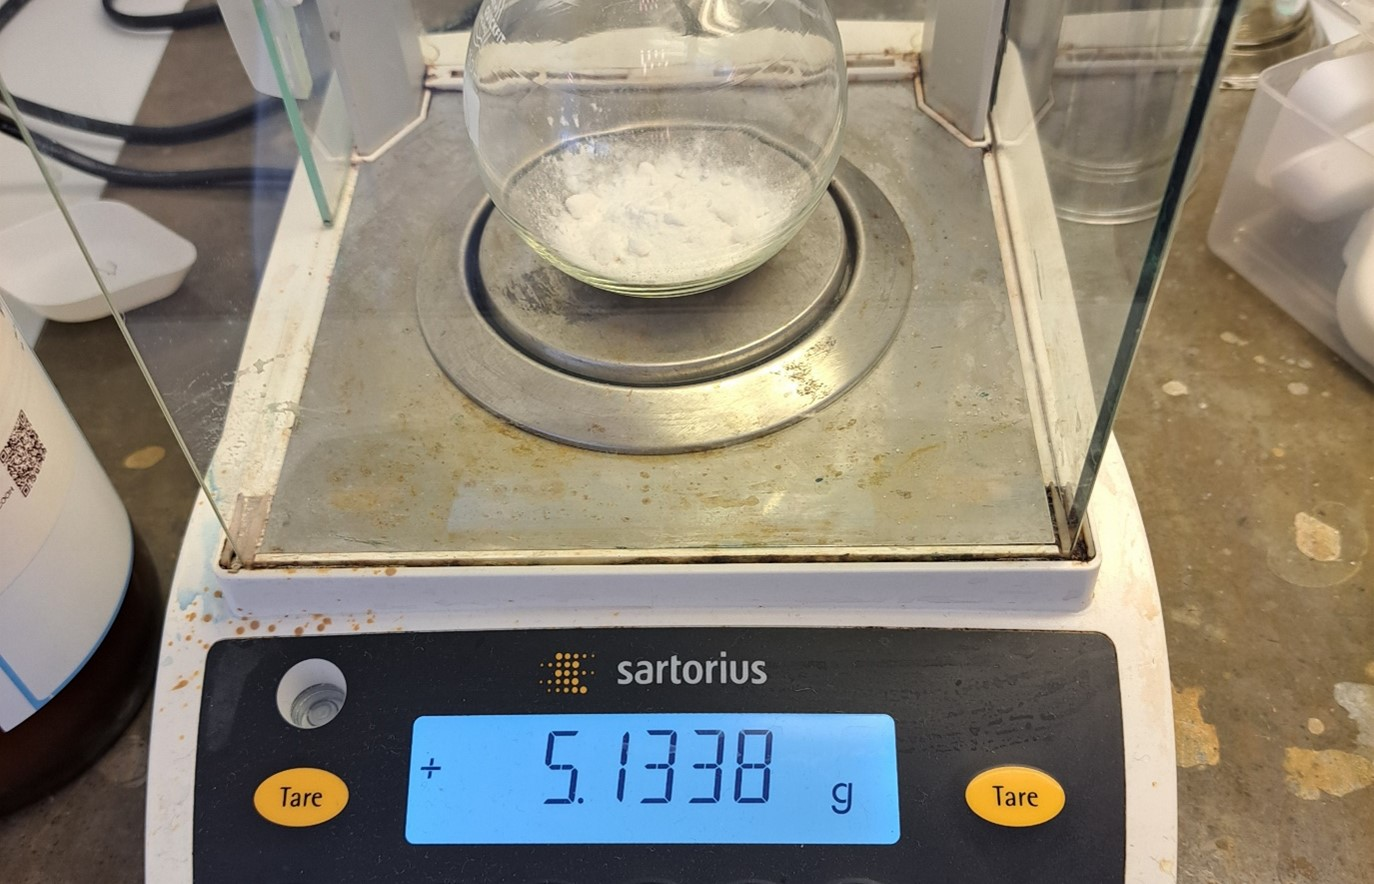
\includegraphics[width=\textwidth]{billeder/afvejning}
        \caption{Afvejning af 4-hydroxybenzoesyre.}
    \end{figure} 
    Da syntesen sker med et overskud af alkohol vil der ideelt ske en fuldstændig reaktion. På baggrund heraf bestemmes det teoretiske udbytte ved at sætte dets stofmængde lig stofmængden af 4-hydroxybenzoesyre:
    \[
        n_{\text{4-hydroxybenzoesyre}}=\frac{5.1338\si{g}}{138.12\si{g \per mol}}=0.037169\si{mol}=n_{\text{ethylparaben}}
    \]
    Den teoretiske stofmængde af dannet ethylparaben omregnes nu til en masse hvorved det fås at:
    \[
        m_{\text{ethylparaben}}=0.037169\si{mol} \cdot 166.17\si{g\per mol}=6.1745g
    \]
    Et regneark udarbejdes til bestemmelsen af det teoretiske udbytte gennem de resterende synteser, en version med værdierne for denne syntese kan ses i bilag 2.

    Der afmåles nu 30mL ethanol i måleglas, hvorefter det overføres til den rundbundede kolbe. Kolben rystes til 4-hydroxybenzoesyren er fuldstændigt opløst, hvorefter 2.5mL svovlsyre tilsættes dråbevist under konstant forsigtig omrystning. Opløsningen placeres i en varmekappe og forsynes med et svalerør for at koge med reflux i ca. 1 time.

    Efter timen er gået slukkes varmekappen, hvorefter opløsningen nedkøles indtil det ikke længere er kogende og overføres til et 250mL bægerglas med 75mL demineraliseret vand. Bægerglasset placeres nu på en kogeplade og tilsættes en magnetomrører, hvorefter der sørges for moderat omrøring. Blandingen bestående af 10\% natriumcarbonat tilsættes nu opløsningen indtil udviklingen af gas stopper, hvorved svovlsyren vil være neutraliseret.

    Idet det ikke indgår i forsøgsvejledningen, udregnes mængden af natriumcarbonat der villet være nødvendig for at neutralisere svovlsyren, dog vil der under processen gøres brug af natriumcarbonat i overskud da det ingen negativ virkning vil have, eftersom temperaturen vil være for lav til at forsæbning af parabenen vil kunnet ske.

    Da svovlsyre har mulighed for at afgive 2 hydroner hvorved det reduceres til dets syrerest-ion, $\mathrm{SO_4^{2-}}$, må den tilsatte base kunnet optage 2 hydroner for at netrualisere 1 svovlsyremolekyle:
    \begin{figure}[H]
        \resizebox{\textwidth}{!}{
        \schemestart
        \chemfig{S(=[1]O)(=[3]O)(-[5]OH)(-[7]OH)}
        \+
        \chemfig{O(-[1]H)(-[7]H)}
        \arrow{->}
        \chemfig{S(=[1]O)(=[3]O)(-[5]OH)(-[7]O^{-})}
        \+
        \chemfig{H^{+}}
        \arrow{->}
        \chemfig{S(=[1]O)(=[3]O)(-[5]O^{-})(-[7]O^{-})}
        \+ 2
        \chemfig{H^{+}}
        \schemestop
        }
        \caption{Dissociering af svovlsyre ved tilsættelse til vand.}
    \end{figure}
    Samtidig er det klart at natriumcarbonat har mulighed for at optage 2 hydroner da det ved tilsættelse til vand øjeblikkeligt dissocierer til natrium- og carbonationer, der herefter reagerer videre for at danne natriumhydroxid.
    \begin{figure}[H]
        \resizebox{\textwidth}{!}{
        \schemestart
        \chemfig{C(=[2]O)(-[5]NaO)(-[7]ONa)}
        \+
        \chemfig{O(-[1]H)(-[7]H)}
        \arrow{->}
        \chemfig{C(-[3]O^{-})(-[5]O^{-})=O}
        \+ 2
        \chemfig{Na^{+}}
        \schemestop
        }
        \caption{Dissociering af natriumcarbonat ved tilsættelse til vand.}
    \end{figure}
    Carbonationen har mulighed for at reagere med vand hvorved der dannes bicarbonat og en hydroxidion, bicarbonationen reagerer videre med vand for at danne ustabil kulsyre og endnu en hydroxidion, hvorefter den ustabile kulsyre brydes hvilket medfører dannelsen af carbondioxid og vand. 
    \begin{align}
        \mathrm{CO_3^{2-} + H_2O} &\longrightarrow \mathrm{HCO_3^- + OH^-} \\
        \mathrm{HCO_3^- + H_2O} &\longrightarrow \mathrm{H_2CO_3 + OH^-} \\
        \mathrm{H_2CO_3} &\longrightarrow \mathrm{CO_2 + H_2O}
    \end{align}
    De dannede hydroxidioner har nu mulighed for at reagere med hydronerne dannet af svovlsyren, mens natriumionerne har mulighed for at reagere med sulfationerne.
    \begin{align*}
        \mathrm{OH^- + H^}+ &\longrightarrow \mathrm{H_2O} \\
        \mathrm{2Na^+ + SO_4^{2-}} &\longrightarrow \mathrm{Na_2SO_4}
    \end{align*}
    Dette muliggør opskrivning som en totalreaktion ved:
    \begin{figure}[H]
        \resizebox{\textwidth}{!}{
        \schemestart
        \chemfig{C(=[2]O)(-[5]NaO)(-[7]ONa)}
        \+
        \chemfig{S(=[1]O)(=[3]O)(-[5]OH)(-[7]OH)}
        \arrow{->}
        \chemfig{S(-ONa)(-[4]NaO)(=[2]O)(=[6]O)}
        \+
        \chemfig{C(=O)(=[4]O)}
        \+ 2
        \chemfig{O(-[7]H)(-[1]H)}
        \schemestop
        }
        \caption{Totalreaktion mellem svovlsyre og natriumcarbonat i vandig opløsning.}
    \end{figure}
    Da det nu er klart at reaktionen mellem svovlsyre og natriumcarbonat foregår i forholdet 1:1 og at der under syntesen benyttes 2.5mL svovlsyre med en densitet på $1.84\si{g \per mL}$ må det være nødvendigt at bruge:
    \[
        n_{\text{svovlsyre}}=\frac{2.5\si{mL} \cdot 1.84\si{g\per mL}}{98.08\si{g\per mol}}=0.04690mol
    \]
    natriumcarbonat til at neutralisere svovlsyren. Stofmængden omregnes til en masse af natriumcarbonat, her er det vigtigt at pointere at der benyttes natriumcarbonatdecahydrat under fremstillingen af opløsningen, grundet dets effekt på molvægten.
    \[
        m_{\text{natriumcarbonat}}=0.04690\si{mol} \cdot 286.14\si{g\per mol}=13.4200\si{g}
    \]
    Da det ikke skaber et problem at tilsætte natriumcarbonat i overskud laves opløsning ved brug af 15g natriumcarbonatdecahydrat og 135g vand. En 10\% opløsning benyttes for at reducere voldsomheden af reaktionen mellem den stærke syre og base, samt for at modvirke dens store eksotermicitet.

    Den neutraliserede opløsning sugefiltreres og skylles 3 gange med demineraliseret vand efter kort tids afkøling. Det isolerede krystallinske stof overføres til et 250mL bægerglas. Samtidigt opvarmes 50mL hhv.\ ethanol og vand til opvarmning i hvert deres bægerglas. Når ethanolen koger opløses det krystallinske stof i så lidt som muligt hvorefter varmt vand tilsættes til opløsningen bliver uklar.

    Opløsningen stilles nu til frivillig nedkøling, hvorved parabenen igen udfældes og kan isoleres ved sugefiltrering i afvejet glasfilterdigel. Det dannede produkt stilles til tørring i glasfilterdiglen benyttet til filtreringen.

    \subsubsection{Syntese 2: Propylparaben}
    

    \subsubsection{Syntese 3: Dobbeltsyntese}
        

    \subsection{Smeltepunktsbestemmelse}
    

    \subsection{NMR--spektroskopi}
    

    \subsection{IR--spektroskopi}
    

    \subsection{Hæmningsforsøg}
    

    \subsubsection{Mueller--Hinton}
    Et hæmningsforsøg udføres også for at undersøge parabenernes hæmmende vækst på forskellige bakterier. Til dette formål vælges det at undersøge 3 forskellige bakterier:
    \begin{table}[H]\centering
        \caption{Karakteristika og navn på udvalgte baktierier.}
        \begin{tabular}{ccc}
            \toprule
            Bakterieart & Cellevægsstruktur \\
            \midrule
            \textit{bacilius cereus} & Gram--positiv \\
            \textit{escherichia coli} & Gram--negativ \\
            \textit{serratia marcescnes} & Gram-negativ \\
            \bottomrule
        \end{tabular}
    \end{table}
    Med udgangspunkt i litteraturen er det klart at parabener er mere effektive mod Gram--positive end Gram--negative bakterier \parencite{Joao2021}. Derudover har tidligere studier undersøgt de effektive koncentrationer for væksthæmning ved de forskellige parabener for bakteriearterne \parencite{Wies2019}. 
    \begin{table}[H]\centering
        \caption{Effektiv parabenkoncentration for hæmning af relevante bakterier.}
        \begin{tabular}{ccc}
            \toprule
            \multicolumn{3}{c}{Effektiv parabenkoncentration $\left[\si{w\per w}\right]$} \\
            Bakterieart & Ethylparaben & Propylparaben \\
            \midrule
            \textit{bacilius cereus} &  0.1 & 0.125 \\
            \textit{escherichia coli} & 0.1--0.125 & 0.05--0.1 \\
            \textit{serratia marcescens} & 0.049 & 0.04 \\ 
            \bottomrule
        \end{tabular}
    \end{table}

    \subsubsection{Fortyndingsrække}
